\documentclass[11pt]{article}
\setlength {\textwidth}{180mm} 
\setlength {\textheight}{260mm}
\topmargin=-35.00mm
\oddsidemargin=-10.00mm
\pagestyle{empty}


\usepackage[toc,page]{appendix}
\usepackage{amsmath, amssymb}
\usepackage{bm}% bold math
\usepackage{cancel, caption}
\usepackage{dcolumn}% Align table columns on decimal point
\usepackage{epsfig, epsf}
\usepackage{graphicx,fancyhdr,natbib,subfigure}
\usepackage{lscape, longtable}
\usepackage{hyperref,ifthen}
\usepackage{verbatim}
\usepackage{color}
\usepackage[usenames,dvipsnames]{xcolor}
\usepackage{listings}
%% http://en.wikibooks.org/wiki/LaTeX/Colors



%%%%%%%%%%%%%%%%%%%%%%%%%%%%%%%%%%%%%%%%%%%
%       define Journal abbreviations      %
%%%%%%%%%%%%%%%%%%%%%%%%%%%%%%%%%%%%%%%%%%%
\def\nat{Nat} \def\apjl{ApJ~Lett.} \def\apj{ApJ}
\def\apjs{ApJS} \def\aj{AJ} \def\mnras{MNRAS}
\def\prd{Phys.~Rev.~D} \def\prl{Phys.~Rev.~Lett.}
\def\plb{Phys.~Lett.~B} \def\jhep{JHEP} \def\nar{NewAR}
\def\npbps{NUC.~Phys.~B~Proc.~Suppl.} \def\prep{Phys.~Rep.}
\def\pasp{PASP} \def\aap{Astron.~\&~Astrophys.} \def\araa{ARA\&A}
\def\jcap{\ref@jnl{J. Cosmology Astropart. Phys.}}%
\def\physrep{Phys.~Rep.}

\newcommand{\preep}[1]{{\tt #1} }

%%%%%%%%%%%%%%%%%%%%%%%%%%%%%%%%%%%%%%%%%%%%%%%%%%%%%
%              define symbols                       %
%%%%%%%%%%%%%%%%%%%%%%%%%%%%%%%%%%%%%%%%%%%%%%%%%%%%%
\def \Mpc {~{\rm Mpc} }
\def \Om {\Omega_0}
\def \Omb {\Omega_{\rm b}}
\def \Omcdm {\Omega_{\rm CDM}}
\def \Omlam {\Omega_{\Lambda}}
\def \Omm {\Omega_{\rm m}}
\def \ho {H_0}
\def \qo {q_0}
\def \lo {\lambda_0}
\def \kms {{\rm ~km~s}^{-1}}
\def \kmsmpc {{\rm ~km~s}^{-1}~{\rm Mpc}^{-1}}
\def \hmpc{~\;h^{-1}~{\rm Mpc}} 
\def \hkpc{\;h^{-1}{\rm kpc}} 
\def \hmpcb{h^{-1}{\rm Mpc}}
\def \dif {{\rm d}}
\def \mlim {m_{\rm l}}
\def \bj {b_{\rm J}}
\def \mb {M_{\rm b_{\rm J}}}
\def \mg {M_{\rm g}}
\def \qso {_{\rm QSO}}
\def \lrg {_{\rm LRG}}
\def \gal {_{\rm gal}}
\def \xibar {\bar{\xi}}
\def \xis{\xi(s)}
\def \xisp{\xi(\sigma, \pi)}
\def \Xisig{\Xi(\sigma)}
\def \xir{\xi(r)}
\def \max {_{\rm max}}
\def \gsim { \lower .75ex \hbox{$\sim$} \llap{\raise .27ex \hbox{$>$}} }
\def \lsim { \lower .75ex \hbox{$\sim$} \llap{\raise .27ex \hbox{$<$}} }
\def \deg {^{\circ}}
%\def \sqdeg {\rm deg^{-2}}
\def \deltac {\delta_{\rm c}}
\def \mmin {M_{\rm min}}
\def \mbh  {M_{\rm BH}}
\def \mdh  {M_{\rm DH}}
\def \msun {M_{\odot}}
\def \z {_{\rm z}}
\def \edd {_{\rm Edd}}
\def \lin {_{\rm lin}}
\def \nonlin {_{\rm non-lin}}
\def \wrms {\langle w_{\rm z}^2\rangle^{1/2}}
\def \dc {\delta_{\rm c}}
\def \wp {w_{p}(\sigma)}
\def \PwrSp {\mathcal{P}(k)}
\def \DelSq {$\Delta^{2}(k)$}
\def \WMAP {{\it WMAP \,}}
\def \cobe {{\it COBE }}
\def \COBE {{\it COBE \;}}
\def \HST  {{\it HST \,\,}}
\def \Spitzer  {{\it Spitzer \,}}
\def \ATLAS {VST-AA$\Omega$ {\it ATLAS} }
\def \BEST   {{\tt best} }
\def \TARGET {{\tt target} }
\def \TQSO   {{\tt TARGET\_QSO}}
\def \HIZ    {{\tt TARGET\_HIZ}}
\def \FIRST  {{\tt TARGET\_FIRST}}
\def \zc {z_{\rm c}}
\def \zcz {z_{\rm c,0}}

\newcommand{\ltsim}{\raisebox{-0.6ex}{$\,\stackrel
        {\raisebox{-.2ex}{$\textstyle <$}}{\sim}\,$}}
\newcommand{\gtsim}{\raisebox{-0.6ex}{$\,\stackrel
        {\raisebox{-.2ex}{$\textstyle >$}}{\sim}\,$}}
\newcommand{\simlt}{\raisebox{-0.6ex}{$\,\stackrel
        {\raisebox{-.2ex}{$\textstyle <$}}{\sim}\,$}}
\newcommand{\simgt}{\raisebox{-0.6ex}{$\,\stackrel
        {\raisebox{-.2ex}{$\textstyle >$}}{\sim}\,$}}

\newcommand{\Msun}{M_\odot}
\newcommand{\Lsun}{L_\odot}
\newcommand{\lsun}{L_\odot}
\newcommand{\Mdot}{\dot M}

\newcommand{\sqdeg}{deg$^{-2}$}
\newcommand{\lya}{Ly$\alpha$\ }
%\newcommand{\lya}{Ly\,$\alpha$\ }
\newcommand{\lyaf}{Ly\,$\alpha$\ forest}
%\newcommand{\eg}{e.g.~}
%\newcommand{\etal}{et~al.~}
\newcommand{\lyb}{Ly$\beta$\ }
\newcommand{\cii}{C\,{\sc ii}\ }
\newcommand{\ciii}{C\,{\sc iii}]\ }
\newcommand{\civ}{C\,{\sc iv}\ }
\newcommand{\SiIV}{Si\,{\sc iv}\ }
\newcommand{\mgii}{Mg\,{\sc ii}\ }
\newcommand{\feii}{Fe\,{\sc ii}\ }
\newcommand{\feiii}{Fe\,{\sc iii}\ }
\newcommand{\caii}{Ca\,{\sc ii}\ }
\newcommand{\halpha}{H\,$\alpha$\ }
\newcommand{\hbeta}{H\,$\beta$\ }
\newcommand{\hgamma}{H\,$\gamma$\ }
\newcommand{\hdelta}{H\,$\delta$\ }
\newcommand{\oi}{[O\,{\sc i}]\ }
\newcommand{\oii}{[O\,{\sc ii}]\ }
\newcommand{\oiii}{[O\,{\sc iii}]\ }
\newcommand{\heii}{[He\,{\sc ii}]\ }
\newcommand{\nv}{N\,{\sc v}\ }
\newcommand{\nev}{Ne\,{\sc v}\ }
\newcommand{\neiii}{[Ne\,{\sc iii}]\ }
\newcommand{\aliii}{Al\,{\sc iii}\ }
\newcommand{\siiii}{Si\,{\sc iii}]\ }


%%%%%%%%%%%%%%%%%%%%%%%%%%%%%%%%%%%%%%%%%%%%%%%%%%%%%
%              define Listings                       %
%%%%%%%%%%%%%%%%%%%%%%%%%%%%%%%%%%%%%%%%%%%%%%%%%%%%%
\definecolor{dkgreen}{rgb}{0,0.6,0}
\definecolor{gray}{rgb}{0.5,0.5,0.5}
\definecolor{mauve}{rgb}{0.58,0,0.82}

\lstset{frame=tb,
  language=Python,
  aboveskip=3mm,
  belowskip=3mm,
  showstringspaces=false,
  columns=flexible,
  basicstyle={\small\ttfamily},
  numbers=none,
  numberstyle=\tiny\color{gray},
  keywordstyle=\color{blue},
  commentstyle=\color{dkgreen},
  stringstyle=\color{mauve},
  breaklines=true,
  breakatwhitespace=true,
  tabsize=3
}

\begin{document}

\title{A Research Note into Dust, Quasar and Host galaxy... }
\author{Nicholas P. Ross and John Timlin}
\date{\today}
\maketitle


\begin{abstract}
This is a Research Note into the properties, observations and physical 
processess associated with dust in Quasars and their host galaxies.
\end{abstract}

\section{Motivation}
``Dust'' - to be defined in due course, is a key astrophysical entity, 
responsible for aiding star formation, emitting mid-infrared electromagnetic
radiation and for obscuring optical light. In particular, we are interested in 
the dust that contributes to an obscuring medium, possibly a torus in a 
Active Galactic Nucleus central engine. We are also keen to related this 
AGN/QSO dust to that of the AGN host galaxy. 

\section{Glossary of Terms}
\begin{table}[h]
\begin{center}
\begin{tabular}{llcl}
\hline
\hline
Term                 & Definition                       &Units & Ref \\
\hline
                         & & & \\
$A(V)$               &  total extinction & magnitudes & Wikipedia\\
                         & total absorption in magnitudes at $V$ & mags & [1] \\
                         & & & \\
$E(B-V)$            & (interstellar) Reddening  & unitless & \\
                          & Color Excess                  &   & Wikipedia \\
                          & $A(B)-A(V)$                    &      &  \\
                          & & & \\
$R(V)$                 & $A(V)/E(B-V)$ &                     & Wikipedia\\
                           & ratio of total to selective absorption at $V$ &  & [1] \\
                           & & & \\
``low reddening''    & $E(B-V)\lesssim0.2$      & -- & \citet{Ross09} \\
                         & & & \\
\hline
\hline
\end{tabular}
\caption{[1] https://ned.ipac.caltech.edu/help/extinction\_law\_calc.html}
\end{center}
\end{table}



\section{Setting up the Problem}
\href{astro.berkeley.edu/ay216/Lecture05-08.pdf}{astro.berkeley.edu/ay216/Lecture05-08.pdf}\\


\noindent
The (“general”) extinction $A_{\lambda}$ can also be written in terms
of the brightness in magnitudes of a source, but this requires knowing
its distances and luminosity.:
\begin{equation}
m_{\lambda} = M_{\lambda} + 4 \log d - 5 + A_{\lambda}.
\end{equation} 
Instead we use the distance independent ``selective extinction'', which is the additional color excess due to extinction:
\begin{eqnarray}
  E(B-V) & = & A(B)-A(V) \\
             & = & (B-V) - (B-V)_{0}
\end{eqnarray} 
The ``normalized selective extinctio'' at any wavelength is also a
common measure of extinction:
\begin{equation}
  E(\lambda, V) / E(B-V)
\end{equation} 
The ``normalized extinction'': $1/R_{V}$, measures the steepness of
the extinction curve:
\begin{eqnarray}
  R_{V} & = &   A(V) / \left [ A(B)-A(V) \right ] \\
          & = &  A(V) / E(B-V)
\end{eqnarray} 
It is steep in the diffuse ISM: $RV = 3.1±0.2$, shallower in dark clouds: RV 


\section{Definition of Dust}
\citet{Draine03} will be our guide... \\
For our purposes we define ``dust'' as... \\

\subsection{Other Key references}
\citet{Pei92}



\section{Dust Laws} 
``One of the main tools used in the study of dust grain properties is
extinction curves, particularly ultraviolet (UV) extinction curves.''
\citep{Gordom03}.

From e.g. (among others!!) \citet{Gordon03, Glikman12}::\\
%% Gordon, K. D., & Clayton, G. C. 1998, ApJ, 500, 816
%%Gordon, K. D., Clayton, G. C., Misselt, K. A., Landolt, A. U., & Wolff, M. J. 2003, ApJ, 594, 279
SMC\\
LMC\\
Milky Way\\
Calzetti94\\

\begin{table}[h]
  \begin{center}
    \begin{tabular}{llcl}
      \hline
      \hline
      Extinction Curve Data                 & $R_{V}$ value & Reference \\
      \hline
      & & & \\
      SMC Bar Sample                       & 2.74$\pm$0.13  & \citet{Gordon03}\\
      SMC Wing Sample                    & 2.05$\pm$0.17  & \citet{Gordon03}\\
      LMC LMC2 Supershell Sample  & 2.76$\pm$0.09  & \citet{Gordon03}\\
      LMC LMC2 Supershell Sample  & 3.41$\pm$0.06  & \citet{Gordon03}\\
      & & & \\
      SMC Bar (AzV 18)                      & 3.60$\pm$0.73  & \citet{Gordon98}\\
      SMC Bar (AzV 214)                    & 2.75$\pm$0.55  & \citet{Gordon98}\\
      SMC Bar (AzV 398)                    & 2.87$\pm$0.40  & \citet{Gordon98}\\
      SMC Wing (AzV 456)                 & 2.66$\pm$0.16  & \citet{Gordon98}\\
      & & & \\
      \hline
      \hline
    \end{tabular}
    \caption{Notes: Average from Table 2 for the \citet{Gordon03} values; 
``Adopted'' values from \citet{Gordon98}.}
\end{center}
\end{table}






\section{AGN Dust}

\section{``Level 5'' Dusty Disks and the Infrared Emission From AGN}
In ``The Central Engine of Active Galactic Nuclei'', ASP Conference Series, Vol. 373, Xi'an, China, 16-21 October, 2007, eds. L. C. Ho and J.-M. Wang 
http://ned.ipac.caltech.edu/level5/Sept07/Li2/Li\_contents.html


\section{Sublimation and the Temperature Gap}
Published in Theory of Accretion Disks, 1989 \\
E. Sterl Phinney\\
http://ned.ipac.caltech.edu/level5/Phinney/Phinney6.html\\

The rate of sublimation of a dust grain at temperature T is given (in g cm$-2$ s$-1$) by 
\begin{equation}
  Q = \sum_{i} (p_{si}(T)-p_{i})S_{i}(T)\sqrt\frac{m_{i}}{2\pi kT}
\end{equation} 
where the index $i$ runs over all equilibrium gas-phase species (e.g. C, C2, CO, etc. for graphite grains), pi is the partial pressure of species i, Si(T) ~ 1 is the sticking fraction for molecules colliding with the grain surface, and $p_{si}$ is the saturation vapor pressure for species i. The saturation vapor pressure is given by 
\begin{equation}
p_{si} = \zeta_{i}(T)kT\frac{(2\pi m_{i}kT)^{3/2}}{h^{3}}\exp \left[ -\frac{h_0}{kt}-\Delta\right]
\end{equation} 
where $\zeta_{i}$ is the product of the rotational, vibrational, and electronic partition functions for the gas-phase species i, and h0 is the heat of sublimation at zero temperature, on a per atom basis. Delta(T) is a complicated expression involving integrals of the specific heat of the solid (Reif 1965, p. 367). Graphite (h0 / k = 8.58 x 104 K to C, h0 / k = 9.82 x 104 K to C2, h0 / k = 9.45 x 104 K to C3, Kelley 1973) is the most refractory substance (with the exception of Tungsten!); silicate grains have h0 / k appeq 6.6 x 104 K. We have fitted the thermodynamic data and sublimation measurements of graphite in vacuum (Kelley 1973), and find that the saturation vapor pressure of the dominant gas-phase constituent is well fitted by 
\begin{equation}
p_{s} = 6\times10^{15} \exp \left[ -92200 / T \right] \rm{dyn} cm^{-2}
\end{equation} 
 The gas pressure in an alpha accretion disk is 
\begin{eqnarray}
p & = & \frac{GM\dot{M}}{4\pi r^{3} \alpha c_{s}} \\
  &  = & 0.01 \, M_{S}\,\dot{m}\,r^{-3}_{\rm{pc}}\alpha^{-1} \, T_{3}^{-1/2} \rm{dyn} \, cm^{-2}
\end{eqnarray} 
 This pressure is comparable to the pressure ~ 10-2 dyn cm-2 in broad-line clouds. Since the solar abundance of carbon, C/H = 4 x 10-4, the partial pressure of carbon, were it all in the gas phase, would be
\begin{equation}
p_{C}  = 10^{-5} \, M_{S}\,\dot{m}\,r^{-3}_{\rm{pc}}\alpha^{-1} \, T_{3}^{-1/2} \rm{dyn} \, cm^{-2}
\end{equation} 

At radii ~ 1 pc, grains grow at an impressive rate: a / adot ~ 5n9 (a / 0.1 µm) yr; in fact the temperatures and densities are quite similar to those in red-giant winds where interstellar dust is believed to form. [But here the grain and gas temperatures need not be equal: the ratio of a grain's radiative cooling luminosity to the rate at which it exchanges energy with gas via collisions is L/H = 10n11-1 Tg,35 / TH,33/2, where the grain temperature is 103 Tg,3 K and the gas temperature and density are 103 TH,3 and 1011 n11 cm-3, respectively]. However, comparing with equation (7) and equation (9), we see that when the grain temperatures Tg exceed 2000 K, graphite grains will certainly begin to sublimate rather than grow. For Tg > 2100 K, the timescale for sublimation of a 1 µm graphite grain becomes shorter than 103 yr, the timescale on which in could be replenished by inflow. From figure 1, we see that this temperature is reached at ~ 0.3 pc in our fiducial quasar.

When the dust sublimates, the gas loses its primary opacity and coolant. As the temperature rises above ~ 3000 K, most common molecules are destroyed, and the opacity drops precipitously by several orders of magnitude (Alexander et al. 1983). The gas in the interior of the disk is then unable to remain in thermal equilibrium at temperatures 2000 ltapprox T ltapprox 7000 K, and must inevitably heat. Above ~ 104 K, the opacity rises abruptly to near its former level as hydrogen is ionized, providing the gas with a new thermal equilibrium state. Unless there is no warp (or down-scattering of radiation onto the disk from electrons or a jet), the transition disk at r < 0.3 pc is thus constrained by the heating from the central source to be optically thin, with T ~ 104 K, until r ltapprox 0.02 pc, when the incident flux can be carried by optically thick thermal emission, and the temperature will begin to rise above 104 K in the accretion disk. The absence of thermalized emission from material with temperatures 2000 ltapprox T ltapprox 7000 K provides a natural explanation for the minimum in nuLnu at nu = 1014.5 Hz (lambda = 1 µm) observed in almost all quasars (Neugebauer et al. 1989). [The reader may mentally add an accretion disk spectrum to the right of figure 2]. Since in this interpretation the frequency is a universal constant, determined (up to very slowly varying logarithms) by the heats of sublimation and dissociation of dust and molecules, and by the ionization of hydrogen, the minimum in the reradiated nuLnu will always be present, and observable unless filled in by starlight or a non-thermal contribution to the spectrum.

Next

\section{Recent Work}
http://arxiv.org/abs/1308.6517


\begin{figure}
    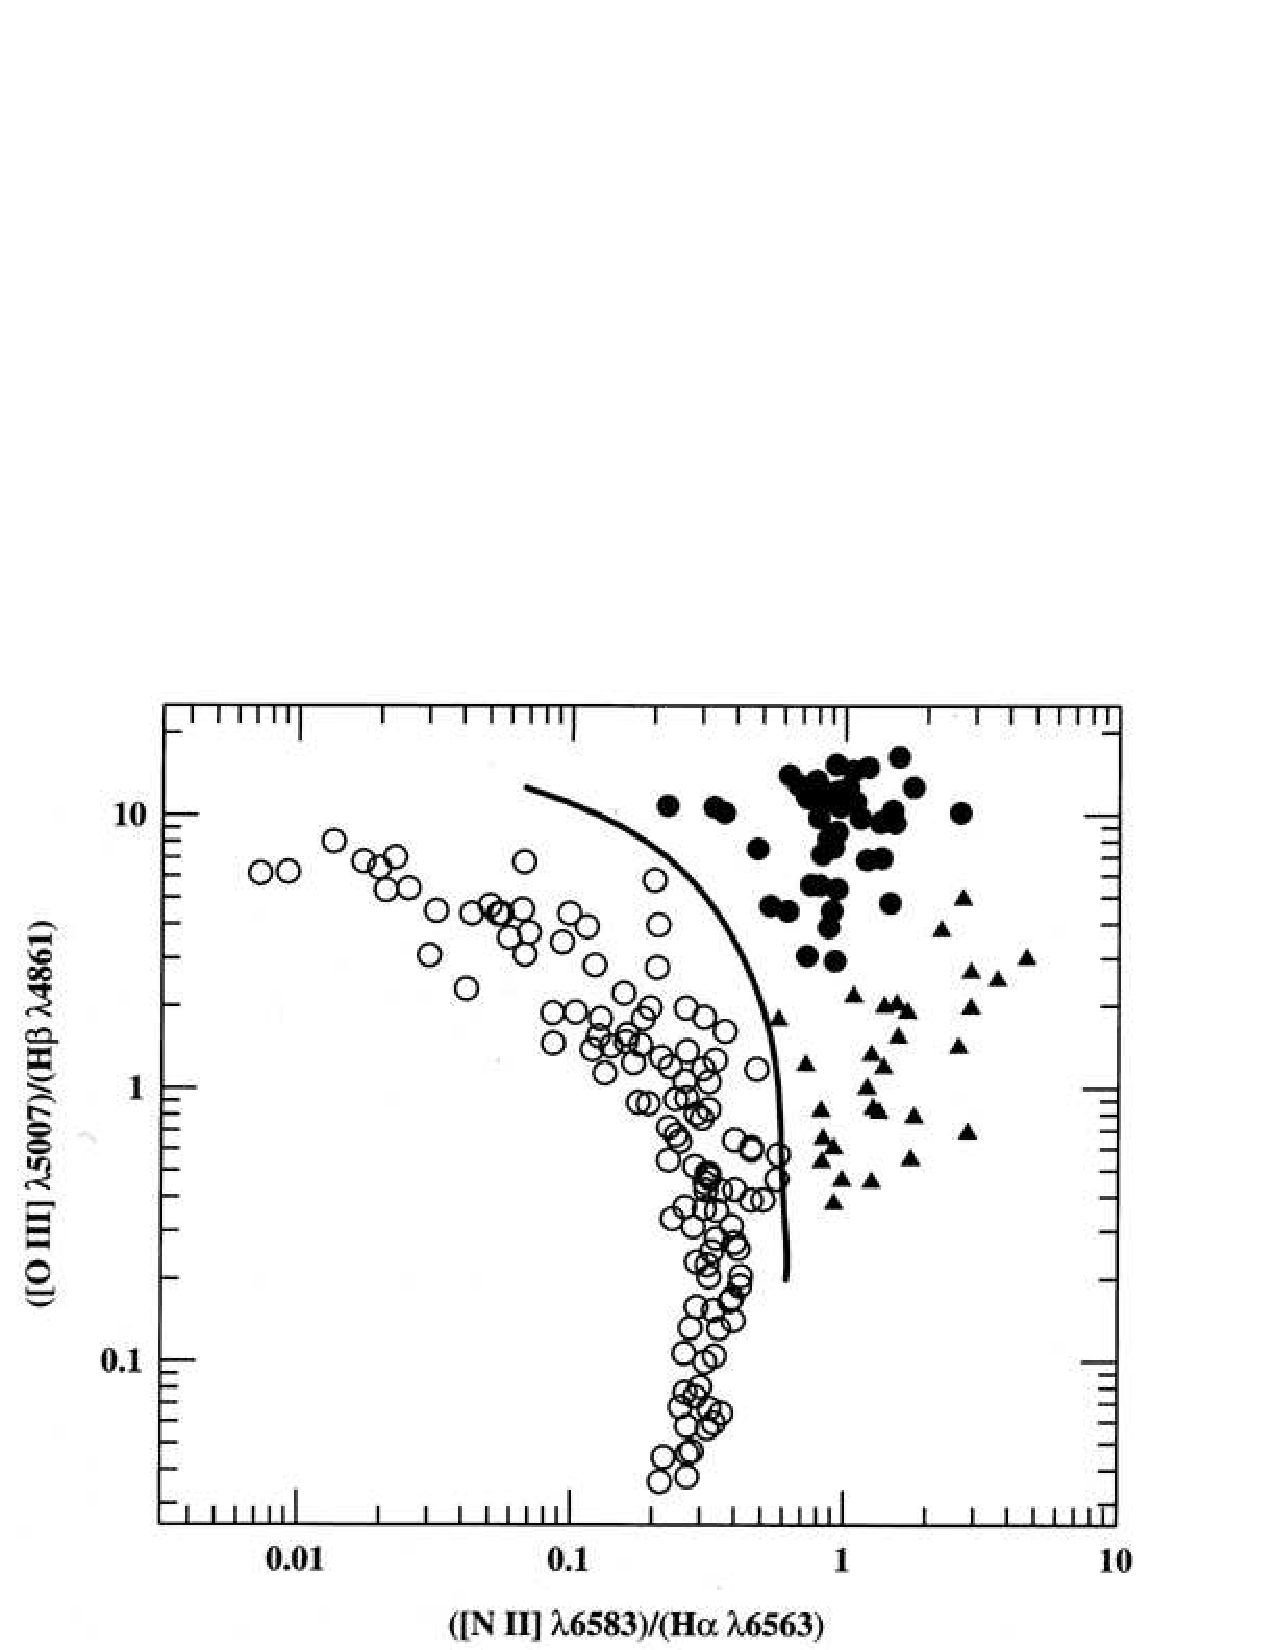
\includegraphics[height=8.0cm,width=6.0cm]
     {BPT.pdf}
     \caption[]{}
\end{figure}
%[O III]/[O II] is sensitive to ionization parameter (how ionized is the gas).
%[O I]/ H $\alpha$ is sensitive to hardness of the radiation field. 

\begin{equation}
A_\lambda/A_I \approx f (\lambda; R_V ,C_1,C_2,C_3,C_4,\lambda_0,\gamma)
%\sigma_{\rm T}= \frac{8\pi}{3} \left(\frac{\alpha\hbar c}{mc^2}\right)^2 = 0.6652\times10^{-24} \,\, \rm{cm}^{-2}
\end{equation}


However, if there is a significant amount of dust associated with the quasar, then the continuum will take on the form:
\begin{eqnarray}
  L_{\lambda},{\rm rest} &\propto& \lambda^{\alpha_{\lambda}} \, e^{-\tau_{\lambda}}\\
  &\propto& \lambda^{\alpha_{\lambda}} \, 10^{-E(B-V) \, R_{\lambda}/2.5}
\end{eqnarray}
where $L_{\lambda},rest$ is the rest frame luminosity, $\alpha_{\lambda}$ is the intrinsic spectral index, $\tau_{\lambda}$ is the optical depth of the dust, and $R_{\lambda}$ is a function that is dependent on the physical properties of the dust.


\newpage

\section{Hugo Messias}
Rayleigh–Jeans law and cut-off in e.g. Fig. 4 of Nenkova et al. 2008, ApJ, 685, 147. 



\newpage


\section{ROE High-$z$ Group: 15th Oct 2014}

    \subsection{Definitions}

    \subsection{Meurer IRX-beta relation}
    e.g. Calzetti et al. 1994\\
    
    
    \subsection{Extinction vs. Attenuation}
    Basically anything outside the MW is Attenuation (and not Extinction!!) \\
    
    \subsection{Meurer IRX-beta relation}
    
    
\section{ROE High-$z$ Group: 03rd Dec 2014 (Loretta Dunne).}
    \subsection{LifeCycle}
    Average timescale for lifecycle is 10$^7$ years...\\
    Condensation temperatue of dust ranges $\sim800-2000$K. \\
    (What's the ``simplest'' type of dust''??!) \\

    \subsection{Dust Sinks}
    Average lifecycle for dust $\sim$10$^8$ years...\\

    \subsection{Questions}
    Chemisty of dust! C vs. Si\\
    and/or Size of dust grains, nm to $\mu$m to few/several $\mu$m\\
    SMG dust properties vs. IMFs vs. sinks and sources (Rowlands'14),    Top Heavy IMFs etc. \\
    Dust in high-$z$ gals (SMGs); high-$z$ QSOs ($z\sim6$)\\
    SNe Explosions, radioactive decay etc. etc. etc. \\
    All this, and how it extrapolates to e.g. the extinction laws... \\
    (really don't know what's going on here!!!) \\
    
    \subsection{References}
    Rowlands et al. (2014)\\
    Gallo et al. (2011? ,2014??)\\
    Hiroshita... 


\section{ROE High-$z$ Group: 11 Feb 2015 (Loretta Dunne).}
Casey, Narayanan and Cooray arXiv:1402.1456v1\\

\section{Useful URLs}
\href{http://etc.stsci.edu/etcstatic/users\_guide/1\_ref\_7\_ebv.html}{http://etc.stsci.edu/etcstatic/users\_guide/1\_ref\_7\_ebv.html}

\section{References}
Draine, 2003, ARAA, 41, 241 \\
Draine 2007 ApJ 663 866 \\
Draine \& Li 2007 ApJ, 657, 810\\
Elitzur, 2006, ApJL, 648, L101 \\
Elitzur, 2006, NewAR, 50, 728 \\
Elitzur, 2008, NewAR, 52, 274 \\
Phinney, 1989, in proc. NATO ASIC Proc. 290: Theory of Accretion Diskstad, Conf, 457 \\
Tielens, 2008, ARAA, 46, 289 \\


\bibliographystyle{mn2e}
\bibliography{/cos_pc19a_npr/LaTeX/tester_mnras}



\end{document}

